
\chapter{Menu Surfaces}
\minitoc 


In most cases, these function only apply on selected surfaces, so, as a prerequisite, you almost always need to select surfaces in order to use what is described below.



\section{Structure modification}
\subsection{Smooth each selected surface}
\noindent
\begin{minipage}{0.5\textwidth}
This option uses vtkSmoothPolyDataFilter.You may smooth an input
selected surface using this option (see Fig. \ref{smooth} p.\pageref{smooth}). A number of iteration and a
relaxation factor are required.\\
See vtkSmoothPolyDataFilter documentation for further information regarding this option.
\end{minipage}    
\begin{minipage}{0.5\textwidth}\centering
  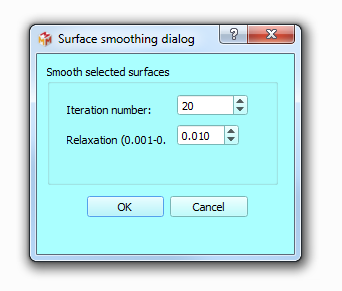
\includegraphics[scale=0.5]{images/09/structure/surface_smoothing_dialog.png}
 \captionof{figure}{Surface smoothing dialog}
 \end{minipage} 
\noindent

\begin{figure}
  \centering
  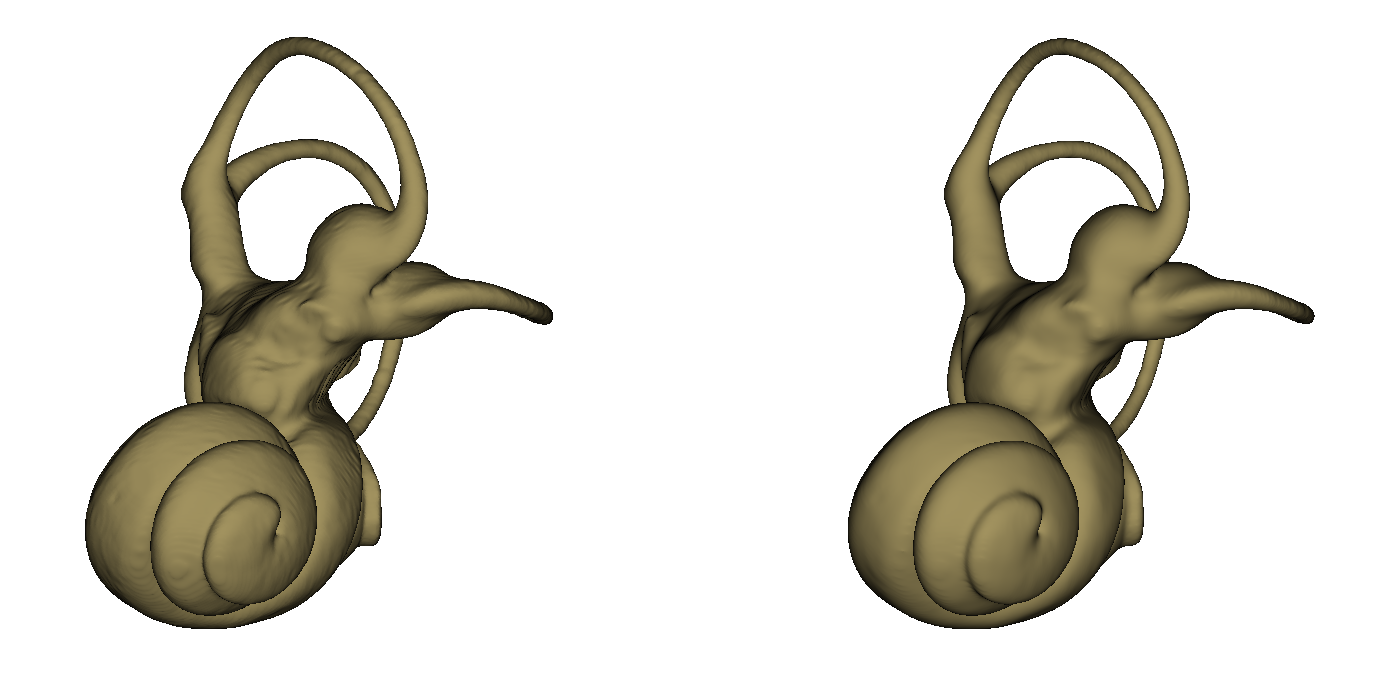
\includegraphics[scale=0.35]{images/09/structure/surface_smoothing_example.png} 
	\caption{Smoothing surfaces. Left: example of original input surface (left inner ear of \textit{Galago moholi}). Right: resulting output surface after 100 iterations using a relaxation factor of 0.1.}
\label{smooth}
 
\end{figure}





\subsection{Decimate each selected surface}
\noindent
\begin{minipage}{0.5\textwidth}


This option uses vtkDecimatePro and vtkQuadricDecimation filters. Requirements : to use mesh decimation, a selected
surface is required (see for instance Fig. \ref{decimate} p.\pageref{decimate}). See vtkDecimatePro and vtkQuadricDecimation documentations for further information regarding
mesh decimation.

\end{minipage}    
\begin{minipage}{0.5\textwidth}\centering
  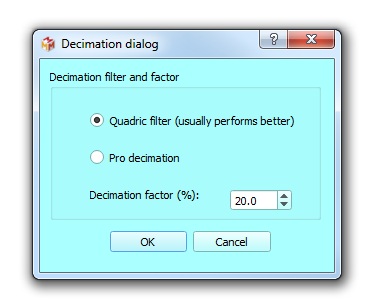
\includegraphics[scale=0.5]{images/09/structure/decimation_dialog.png}
 \captionof{figure}{Decimate window}
 \end{minipage} 
\noindent

\begin{figure}
  \centering
  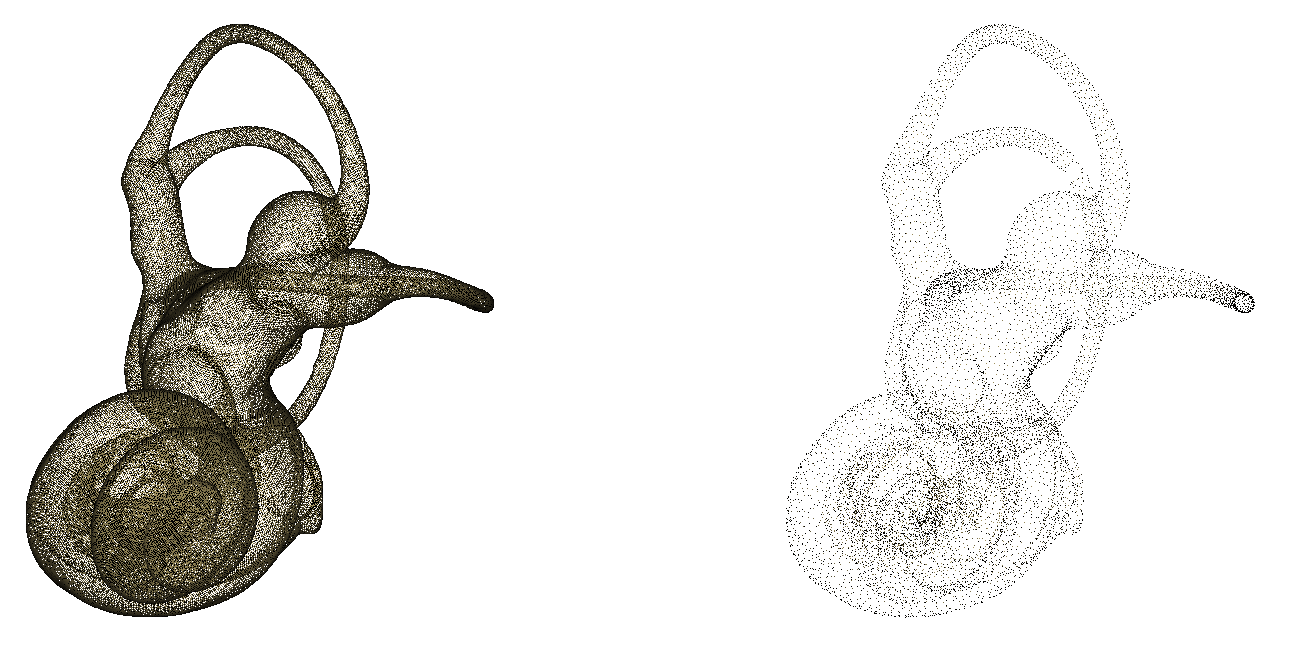
\includegraphics[scale=0.35]{images/09/structure/decimation_example.png} 
	\caption{Surface decimation. Left: point cloud rendering of input surface (left inner ear of \textit{Galago moholi}). Right: point cloud rendering of resulting output (vtkQuadricDecimation filter,
decimation factor: 95\%). 
}
\label{decimate}
 
\end{figure}

\subsection{Densify each selected surface}

\noindent
\begin{minipage}{0.5\textwidth}

This option uses vtkDensifyPolyData filter.
Requirements : to use mesh densification, a selected
surface is required (see for instance Fig. \ref{densify} p.\pageref{densify}).
Note that mesh decimation can become extremely slow
when using number of subdivisions larger than 1.
See vtkDensifyPolyData documentation for further information regarding mesh densification.

\end{minipage}    
\begin{minipage}{0.5\textwidth}\centering
  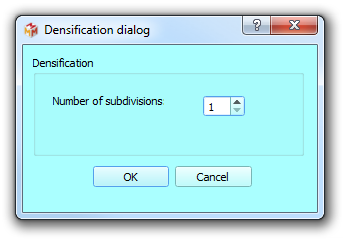
\includegraphics[scale=0.5]{images/09/structure/densification_dialog.png}
 \captionof{figure}{Densify dialog}
 \end{minipage} 
\noindent

\begin{figure}
  \centering
  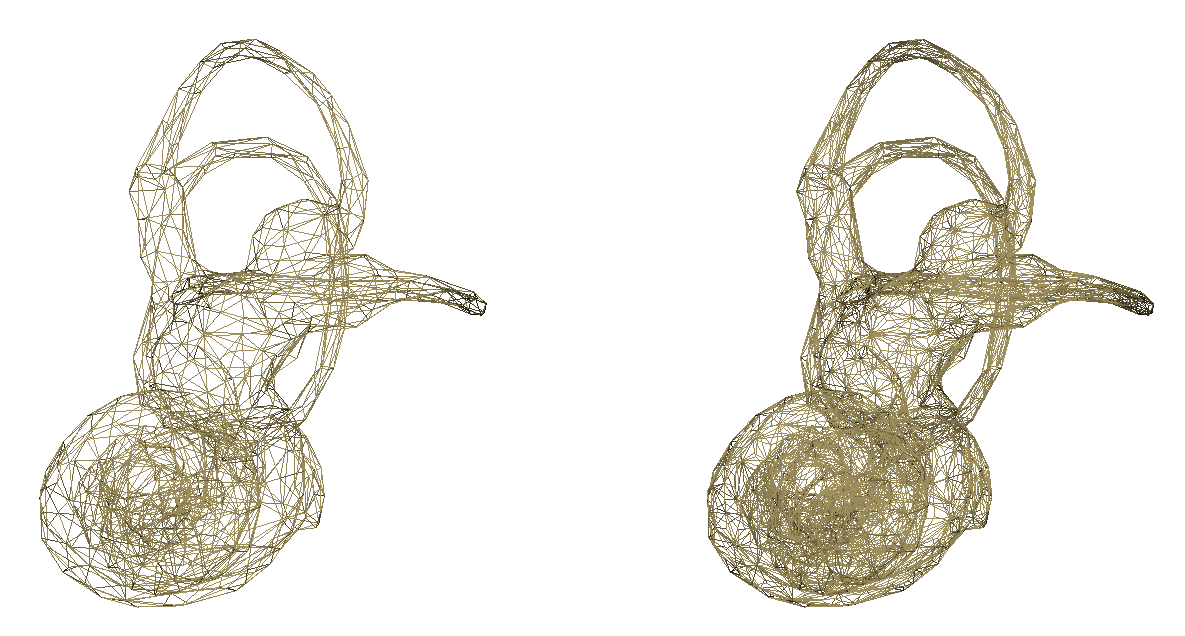
\includegraphics[scale=0.35]{images/09/structure/densification_example.png} 
	\caption{Surface densification. Left: wireframe rendering of input surface (left inner ear of \textit{Galago moholi}). Right: wireframe rendering of resulting output (number of subdivisions: 1).
}
\label{densify}
 
\end{figure}




\subsection{Fill holes of each selected surface}

\noindent
\begin{minipage}{0.5\textwidth}

This option uses vtkFillHolesFilter.
Requirements : to use mesh hole filling, a selected surface is
required (see for instance Fig. \ref{fill_holes} p.\pageref{fill_holes}). See vtkFillHolesFilter documentation for further
information regarding hole filling.


\end{minipage}    
\begin{minipage}{0.5\textwidth}\centering
  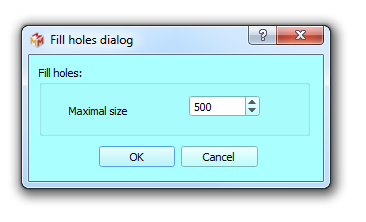
\includegraphics[scale=0.5]{images/09/structure/fill_holes_dialog.png}
 \captionof{figure}{Fill holes window}
 \end{minipage} 
\noindent

\begin{figure}
  \centering
  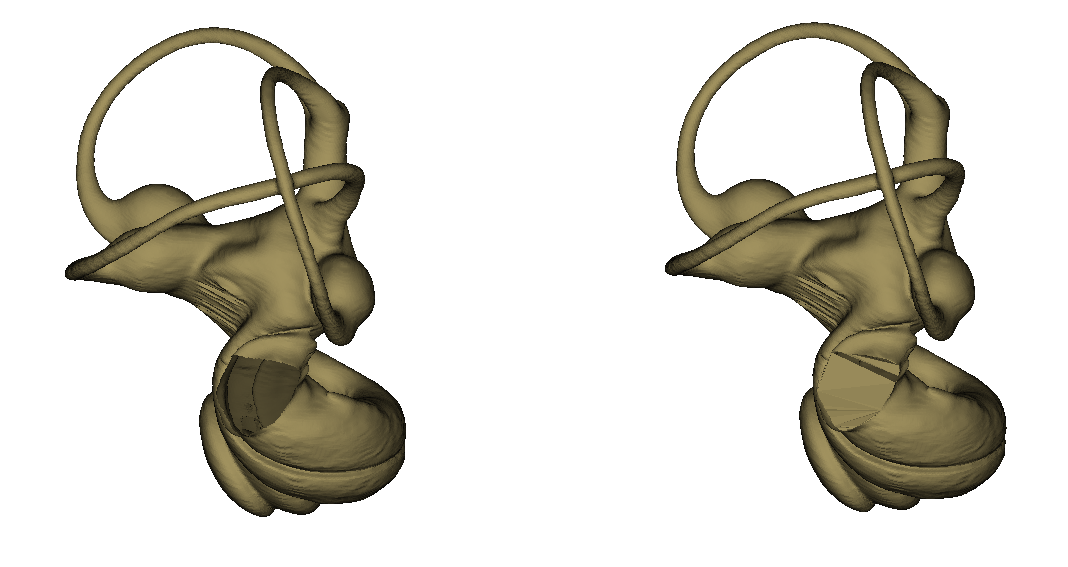
\includegraphics[scale=0.35]{images/09/structure/fill_holes_example.png} 
	\caption{Filling holes. Left: input surface: left inner ear of \textit{Galago moholi} having a hole in the round window. Right: resulting surface output.}
\label{fill_holes}
 
\end{figure}






\subsection{TPS deformation of each selected surface}
\noindent
\begin{minipage}{0.5\textwidth}
This option uses vtkThinPlateSplineTransform filter.
Requirements : to use TPS deformation, a selected surface,
a series of ``n" normal landmarks and a series of ``n"
target landmarks (n>3) are needed. ``Normal" landmarks
are usually placed on the original selected input surface,
whereas ``target" landmarks are placed at a location in 3D
space which will drive the TPS deformation (see Fig. \ref{tps} p.\pageref{tps}). See vtkThinPlateSplineTransform documentation for further information regarding TPS deformation.

\end{minipage}    
\begin{minipage}{0.5\textwidth}\centering
  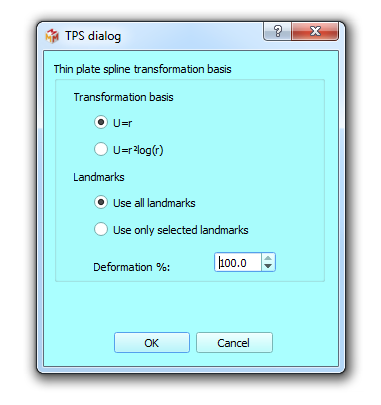
\includegraphics[scale=0.5]{images/09/structure/tps_dialog.png}
 \captionof{figure}{TPS dialog}
 \end{minipage} 
\noindent

\begin{figure}
  \centering
  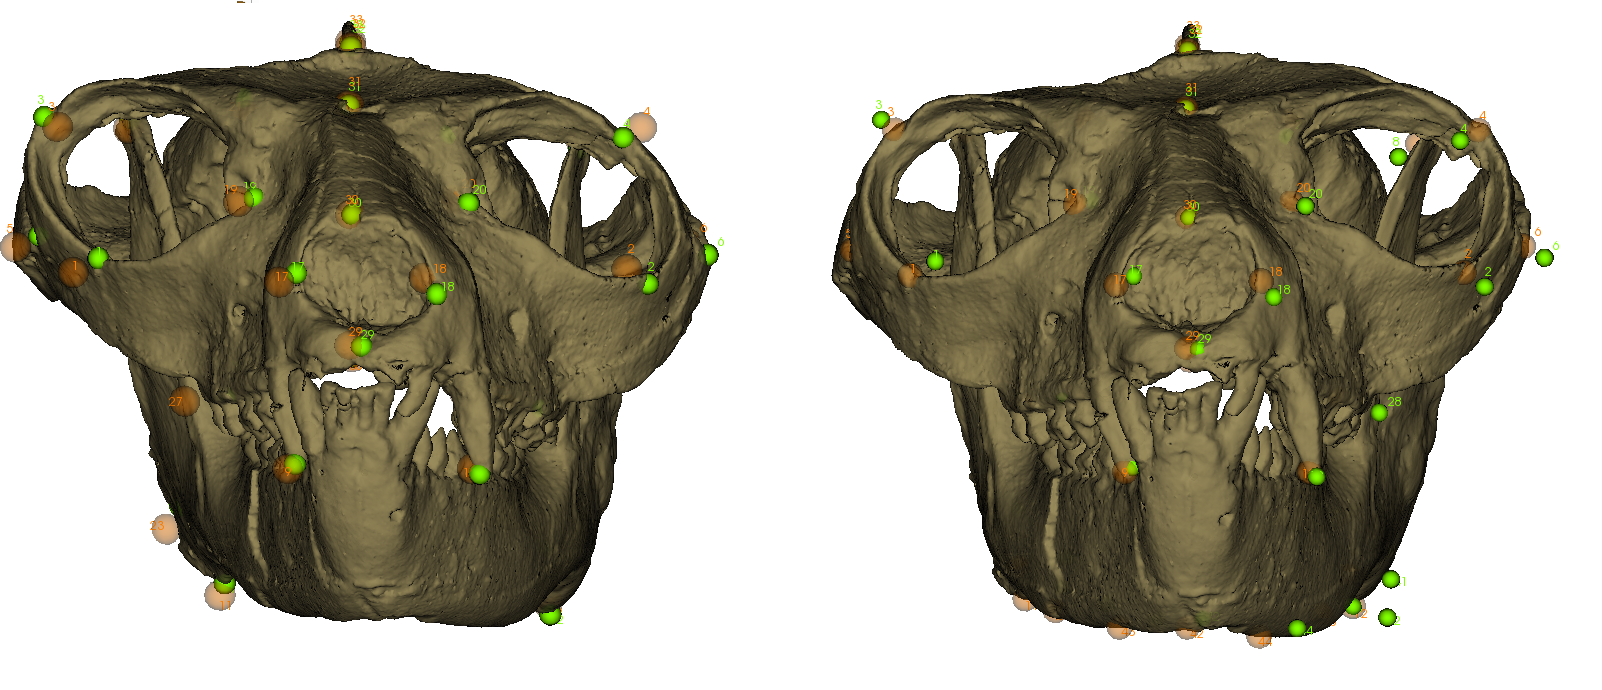
\includegraphics[scale=0.31]{images/09/structure/tps_example.png} 
	\caption{Thin plate spline (TPS) transformation. Left: original distorted input surface of the cranium and mandible of \textit{Notharctus tenebrosus} (3D surface obtained from a cast of specimen AMNH 127167 from the American Museum of Natural History, New York City, New York, USA). 46 ``normal"
landmarks were placed on the surface and 46
``target" landmarks were placed in order to
restore bilateral symmetry. Right: resulting output (deformation : 100\%). Note
that the 46 ``target" landmarks are located on the output surface.
}
\label{tps}
 
\end{figure}




\subsection{Connectivity: separate each selected surface into independent regions}
\noindent
\begin{minipage}{0.5\textwidth}
This option uses vtkPolyDataConnectivityFilter. This filter produces a new surface for each non-connected region of the selected input surface. 3D meshes of biological objects sometimes contain a multitude of small and biologically irrelevant independent regions. This ``noise" may have multiple origins: low quality of original 3D data, state of preservation of the specimen, threshold used to be able to visualize all relevant structures, etc... In order to extract relevant independent regions, only regions reaching a minimal size (minimal number of triangles) are transformed into new surfaces (see Fig. \ref{decompose34} p.\pageref{decompose34}). This process may take some time to be completed. All produced surfaces corresponding to independent regions can be manipulated independently.\end{minipage}    
\begin{minipage}{0.5\textwidth}\centering
  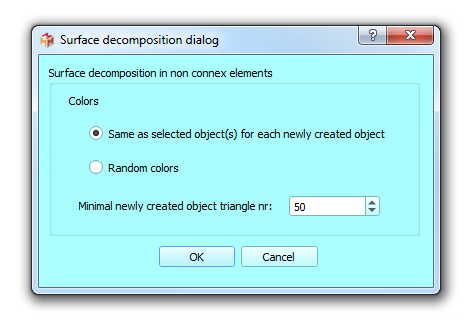
\includegraphics[scale=0.5]{images/09/structure/surface_decomposition_dialog.png}
 \captionof{figure}{Connectivity decomposition dialog}
 \end{minipage} 
\noindent


\begin{figure}
  \centering
  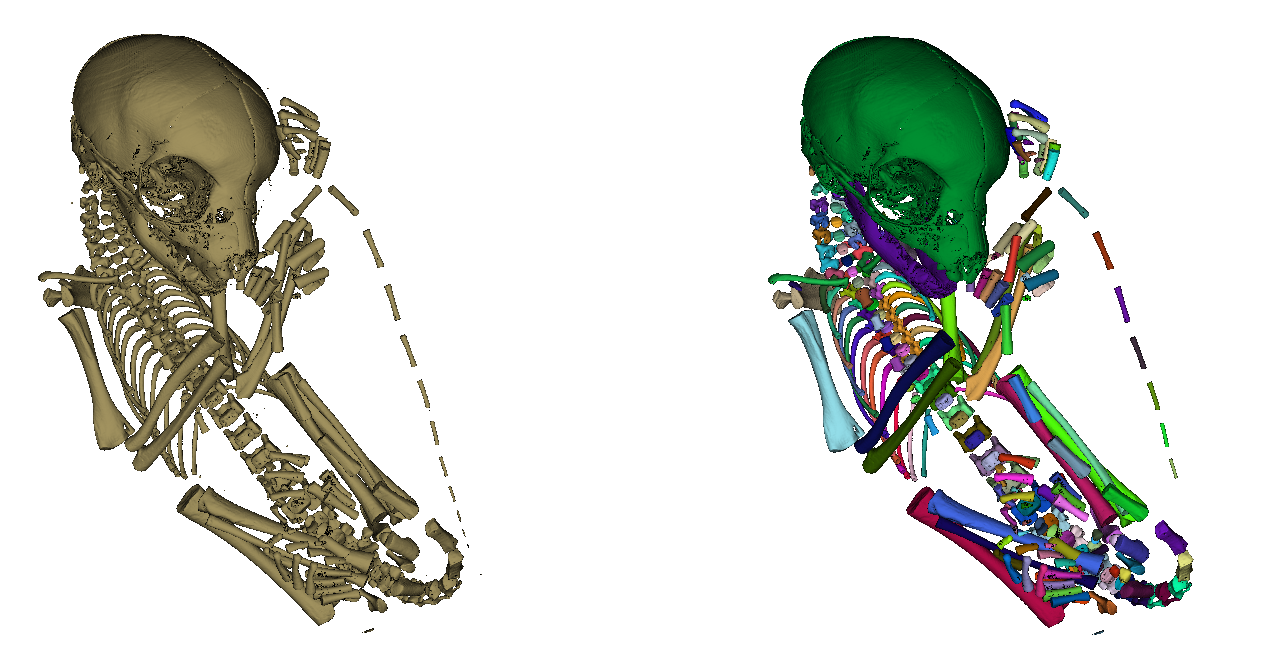
\includegraphics[scale=0.35]{images/09/structure/surface_decomposition_example.png} 
	\caption{Example of surface decomposition into non-connected surfaces. Left: original surface of the skeleton of a newborn \textit{Lemur catta} containing a large number of independent regions of size greater than 500 triangles. Right : Output result (independent surface objects) Filtered surfaces. All surfaces produced using this filter have more than 500 triangles and were given a random color. Note that several bones of the most distal part of the tail are absent, because they contain less than 500 triangles. }
\label{decompose34}
 
\end{figure}






\subsection{Connectivity: keep largest region for each selected surface}
This option uses vtkPolyDataConnectivityFilter.This filter produces a new surface for the largest independent region of the selected input surface (see Fig. \ref{largest_region} p.\pageref{largest_region}).

\begin{figure}
  \centering
  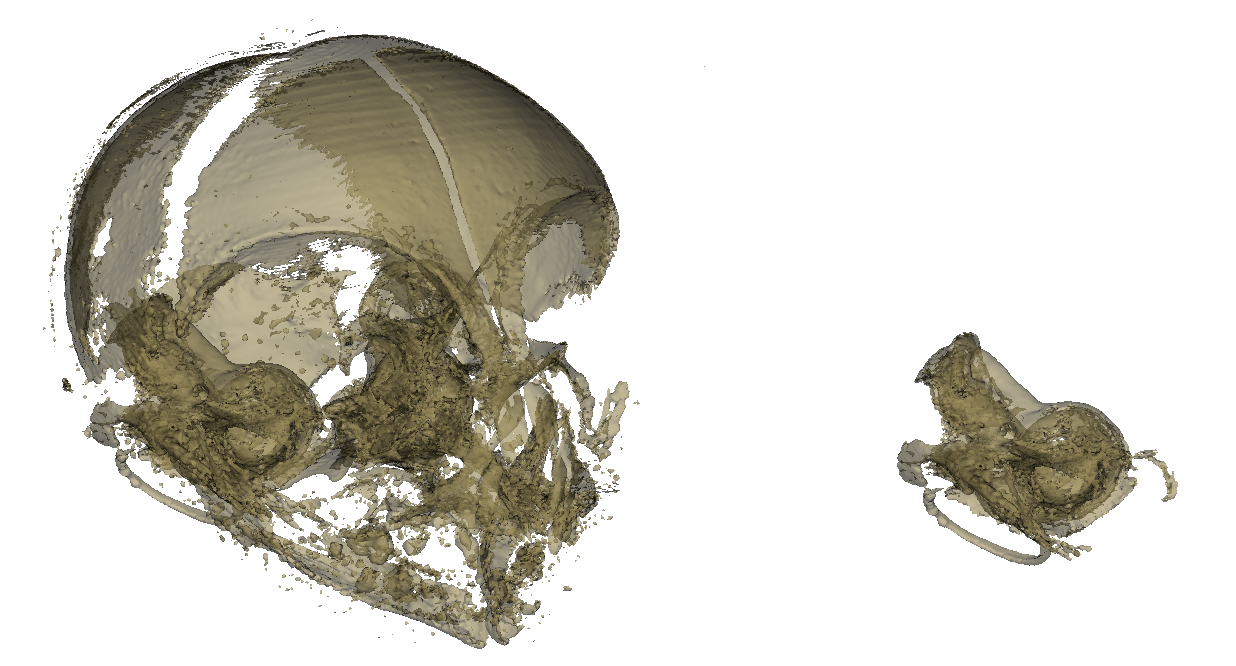
\includegraphics[scale=0.31]{images/09/structure/keep_largest.png} 
	\caption{Example of surface decomposition in order to keep largest region. Left: original 3D surface representing the skull of a newborn \textit{Tarsius bancanus}. Right: the resulting largest region in terms of triangle number.}
\label{largest_region}
 
\end{figure}


\subsection{Invert each selected surface}

A given surface can be inverted in order to show inner structures (see Fig. \ref{inversion} p.\pageref{inversion}).\\


\begin{figure}
  \centering
  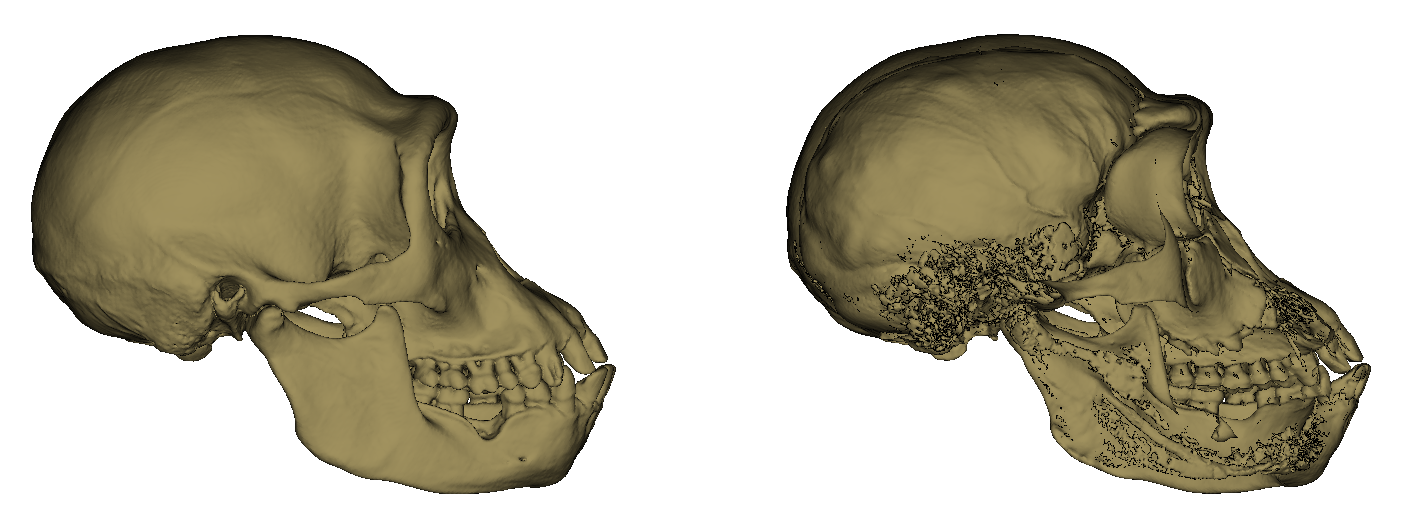
\includegraphics[scale=0.32]{images/09/structure/inversion_example.png} 
	\caption{Example of surface inversion. Left: original surface of the skull of the type specimen of \textit{Pan paniscus}.
Right: backface culling rendering of the same surface after being inverted, revealing inner structures such as the endocranial cavity. }
\label{inversion}
 
\end{figure}

\subsection{Mirror each selected surface along Y plane}

This option uses vtkReflectionFilter, which produces a mirror image of the original selected input mesh (see Fig. \ref{mirror} p.\pageref{mirror}).\\

\begin{figure}
  \centering
  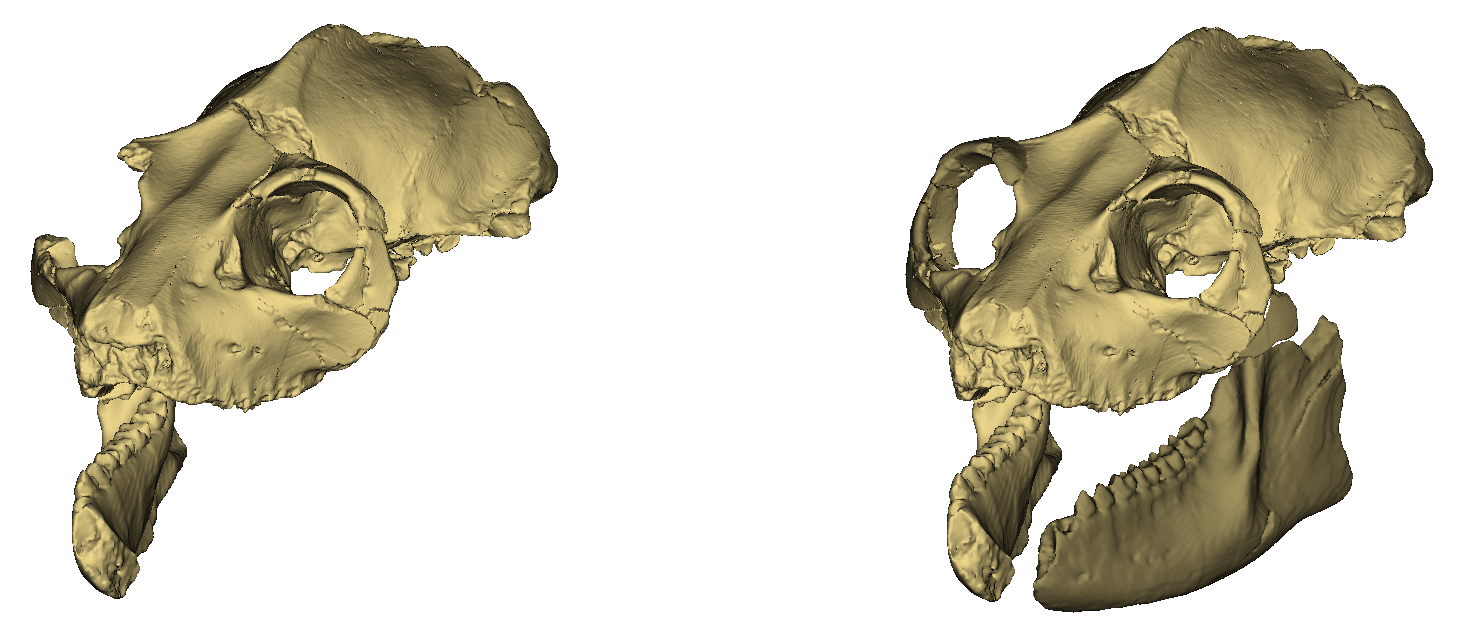
\includegraphics[scale=0.32]{images/09/structure/image_mirror.png} 
	\caption{Example of fossil restoration (\textit{Palaeolemur betillei} BOR613 specimen from the Musée d'Histoire Naturelle de Bordeaux, France) implicating the production of mirror images of missing parts.}
 \label{mirror}
\end{figure}

\subsection{Merge selected surfaces into one single surface}
This options makes it possible to merge all selected surfaces into one single surface object. 


\section{Wrapping methods}
\subsection{Create a convex hull for each selected surface}
This option uses vtkDelaunay3D. This filter produces convex hull surfaces for each selected surface. Convex hulls can be useful for instance to compute estimations of the total "volume" occupied in space by complex objects containing lots of holes (see Fig. \ref{convex_hull} p.\pageref{convex_hull}). 

\begin{figure}
  \centering
  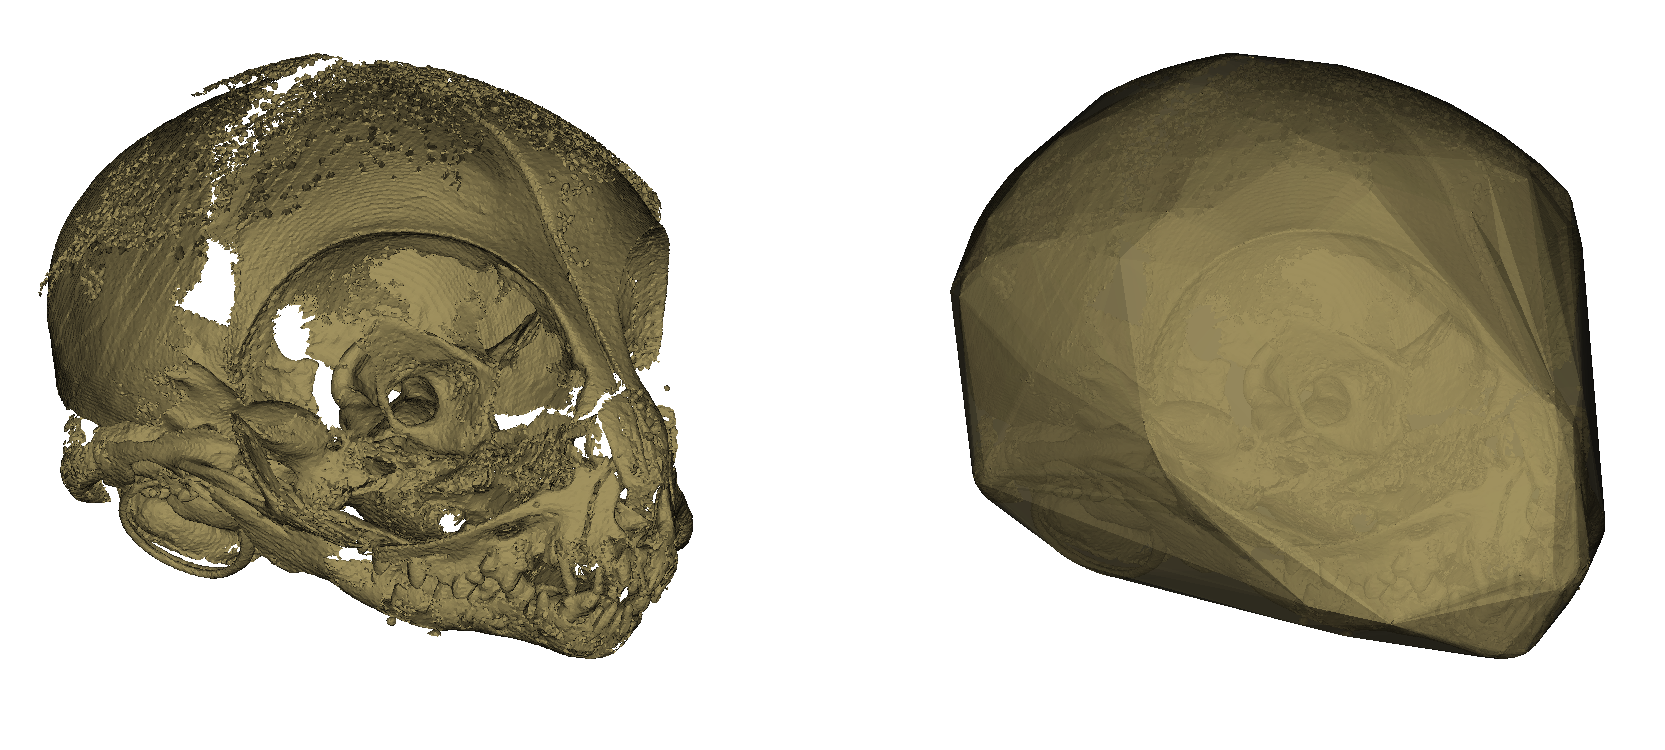
\includegraphics[scale=0.27]{images/09/wrapping_methods/convex_hull.png} 
	\caption{Convex hull computation. \textbf{Left:} original 3D surface representing the skull of a newborn \textit{Tarsius bancanus}. Bone volume: \textasciitilde100 mm3. \textbf{Right:} the resulting convex hull. Volume of the convex hull of the skull (=proxy for the volume of the "head"): \textasciitilde3653 mm3.}
\label{convex_hull}
 
\end{figure}

\subsection{Shrink and wrap 1 surface over a 2nd surface}
This option uses vtkSmoothPolyDataFilter to shrink a surface over the points of a second surface. \textbf{Warning:} the first (=impacted) surface should enclose the second (=observed) surface. This will approximately produce a convex hull of the observed object (see Fig. \ref{shrink_wrap_dialog} p.\pageref{shrink_wrap_dialog} and Fig. \ref{shrink_wrap_example} p.\pageref{shrink_wrap_example}). 

\begin{figure}
  \centering
  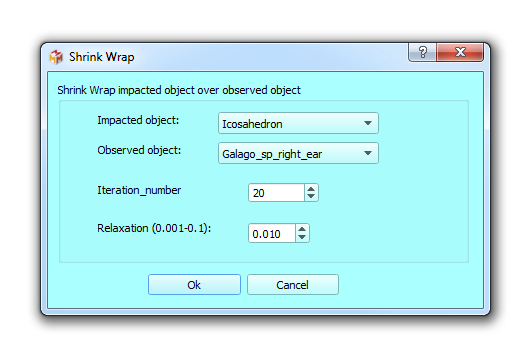
\includegraphics[scale=0.5]{images/09/wrapping_methods/shrink_wrap_dialog.png} 
	\caption{Shrink wrap dialog .}
\label{shrink_wrap_dialog}
 
\end{figure}

\begin{figure}
  \centering
  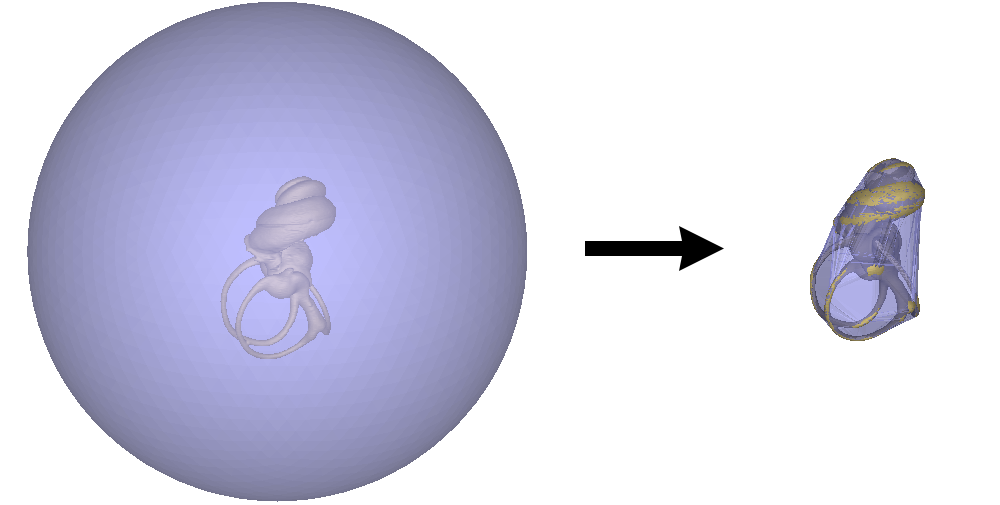
\includegraphics[scale=0.45]{images/09/wrapping_methods/shrink_wrap_example.png} 
	\caption{Convex hull computation. \textbf{Left:} A transparent sphere encloses the 3D surface representing the inner ear of a \textit{Galago moholi} and (level . \textbf{Right:} the sphere was skink-wrapped over the inner ear, resulting approximately in a convex hull.}
\label{shrink_wrap_example}
 
\end{figure}



\section{Surface alignment}\label{surface_alignment_section}
\noindent
\begin{minipage}{0.5\textwidth}
This option uses vtkIterativeClosestPointTransform filter. This filter makes it possible to align two surfaces using the Iterative Closest Point (ICP) algorithm. In order to get good results, it is strongly advised to orient manually roughly the two surfaces in the same direction before running this algorithm 
(see for instance Fig. \ref{surface_alignment} p.\pageref{surface_alignment}). See vtkIterativeClosestPointTransform documentation for further information.



\end{minipage}    
\begin{minipage}{0.5\textwidth}\centering
  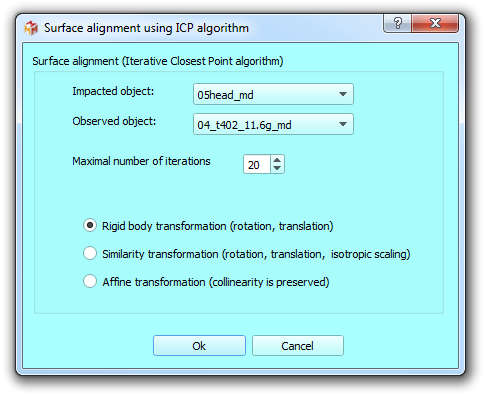
\includegraphics[scale=0.5]{images/09/alignment/surface_alignment_dialog.png}
 \captionof{figure}{Surface alignment dialog}
 \end{minipage} 

\begin{figure}
  \centering
  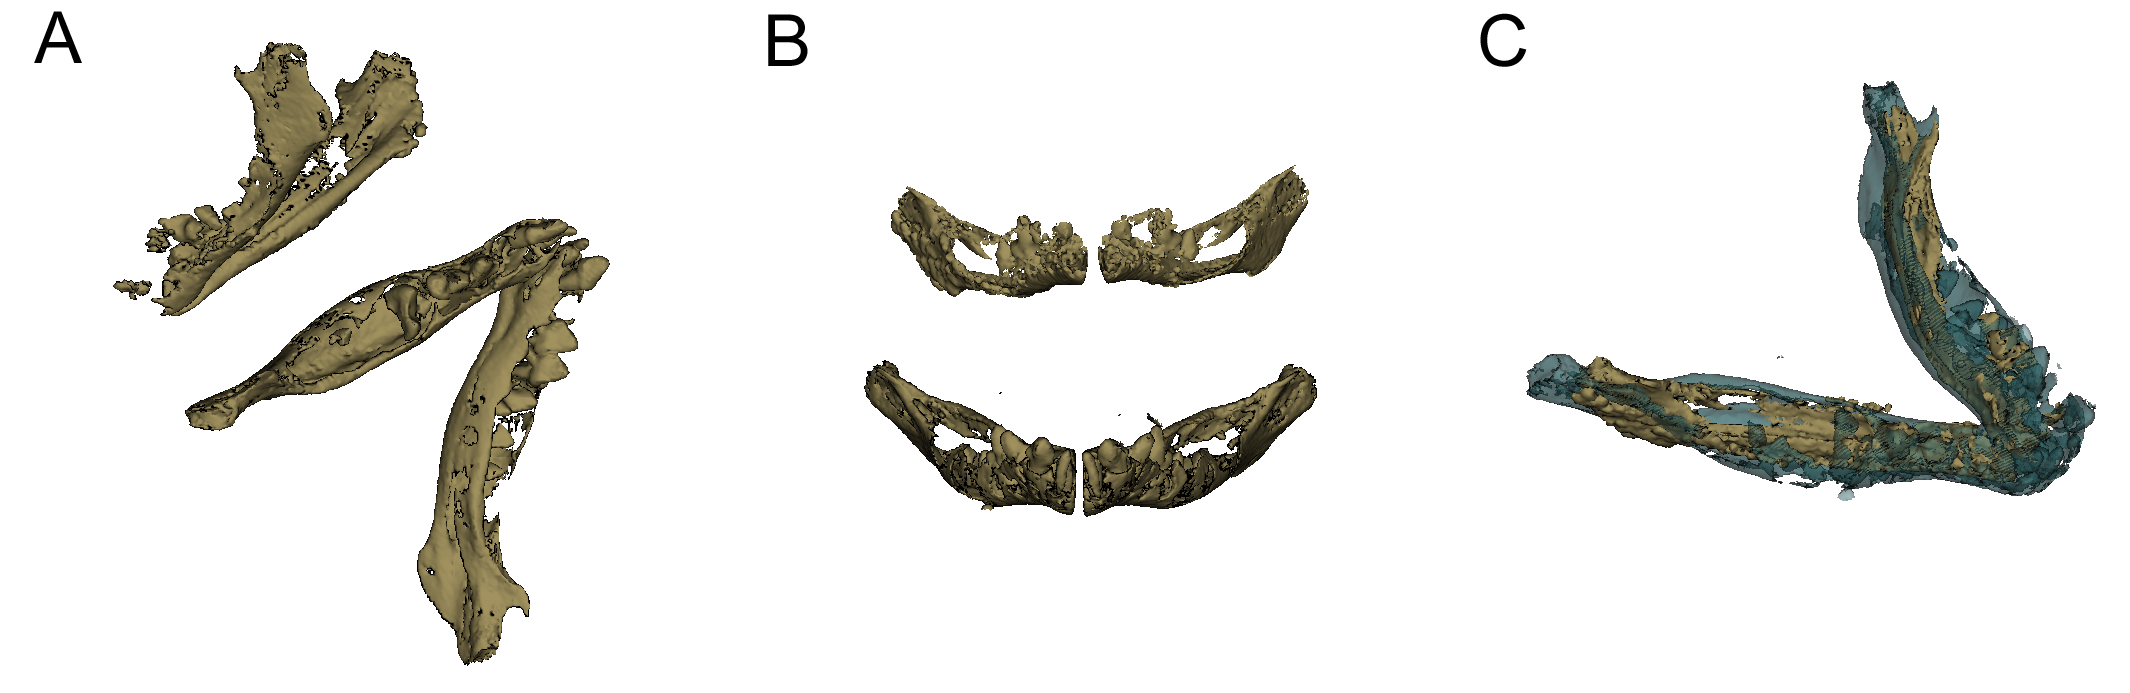
\includegraphics[scale=0.21]{images/09/alignment/surface_alignment.png} 
	\caption{Example of alignment of two mandibles of \textit{Tarsius bancanus}. A: the two surfaces in their initial orientation. B: the two mandibles were roughly manually oriented in the same direction. C: result of the ICP algorithm. The impacted surface (the one which was actually reoriented) is the blue one. }
 \label{surface_alignment}
\end{figure}



\section{Rendering modification}



\subsection{Change transparency}
\noindent
\begin{minipage}{0.4\textwidth}
All selected actors can be given the same transparency using this option (at least one selected surface is needed).\\
Please choose a value between 0 and 100. 100 stands for ``opaque rendering". 0 stands for ``invisible surface".\\


\end{minipage}    
\begin{minipage}{0.6\textwidth}\centering
  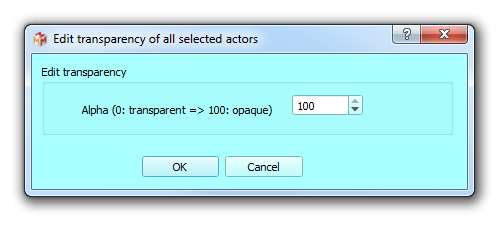
\includegraphics[scale=0.5]{images/09/rendering/transparency.png}
 \captionof{figure}{Edit transparency dialog}
 \end{minipage} 
\noindent





\subsection{Change object solid color}
Selected objects' solid color can be changed using this option. A set of 13 predefined colors is available via this menu. Alternatively, you can edit object color manually using the ``Default solid color of surfaces" control of the ``Edit color options" window (menu ``Edit $\rightarrow$Edit color options").

\section{Create 3D printing connective material}
When planning to print a 3D model composed of non connex elements (for instance : the cranium and the mandible of a single individual, or the skeleton of the fetus of a vertebrate specimen), you may need to manually place in 3D space connective surface elements linking those different parts. Such elements are referred to as "3D printing connective struts", and can be created via the "Cylindric connective struts" dialog (Fig. \ref{cylinders_dialog} p.\pageref{cylinders_dialog}) or via the "Cubic connective struts" dialog (Fig. \ref{cubes_dialog} p.\pageref{cubes_dialog}). 
\subsection{Create cylindric connective struts}
Different options are available, and in particular, the cylinders can be given either conic of flat ends, and the cross-section of the cylinders can either be circular or elliptic (Fig. \ref{conic_non_conic} p.\pageref{conic_non_conic}). 
Two practical examples of 3D printed objects using cylindric connective struts are shown in Fig. \ref{support_example} p.\pageref{support_example}.
\begin{figure}
  \centering
  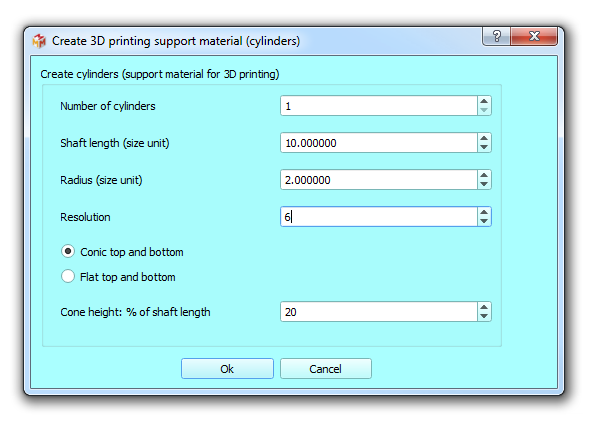
\includegraphics[scale=0.5]{images/09/create_3D_printing_support_surfaces/cylinders_dialog.png} 
	\caption{Create cylinders dialog. Different options are available. Several cylinders sharing the same properties can be created at once. Shaft length and radius can be defined, as well as the resolution (number of sides). Also, shaft section shape can either be circular or elliptical. The bottom and top sides of the cylinders can be either flat, or conic.}
 \label{cylinders_dialog}
\end{figure}

\begin{figure}
  \centering
  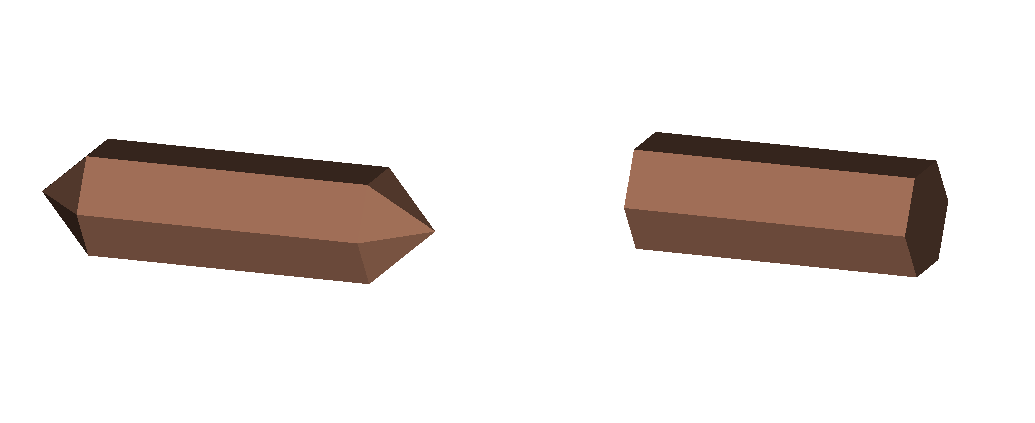
\includegraphics[scale=0.5]{images/09/create_3D_printing_support_surfaces/conic_non_conic.png} 
	\caption{Different cylinder shapes. \textbf{Top left}: flat ends + circular shaft section. \textbf{Top right:} conic ends + circular shaft section. \textbf{Bottom left}: flat ends + elliptical shaft section. \textbf{Top right:} conic ends + elliptical shaft section.}
 \label{conic_non_conic}
\end{figure}

\begin{figure}
  \centering
  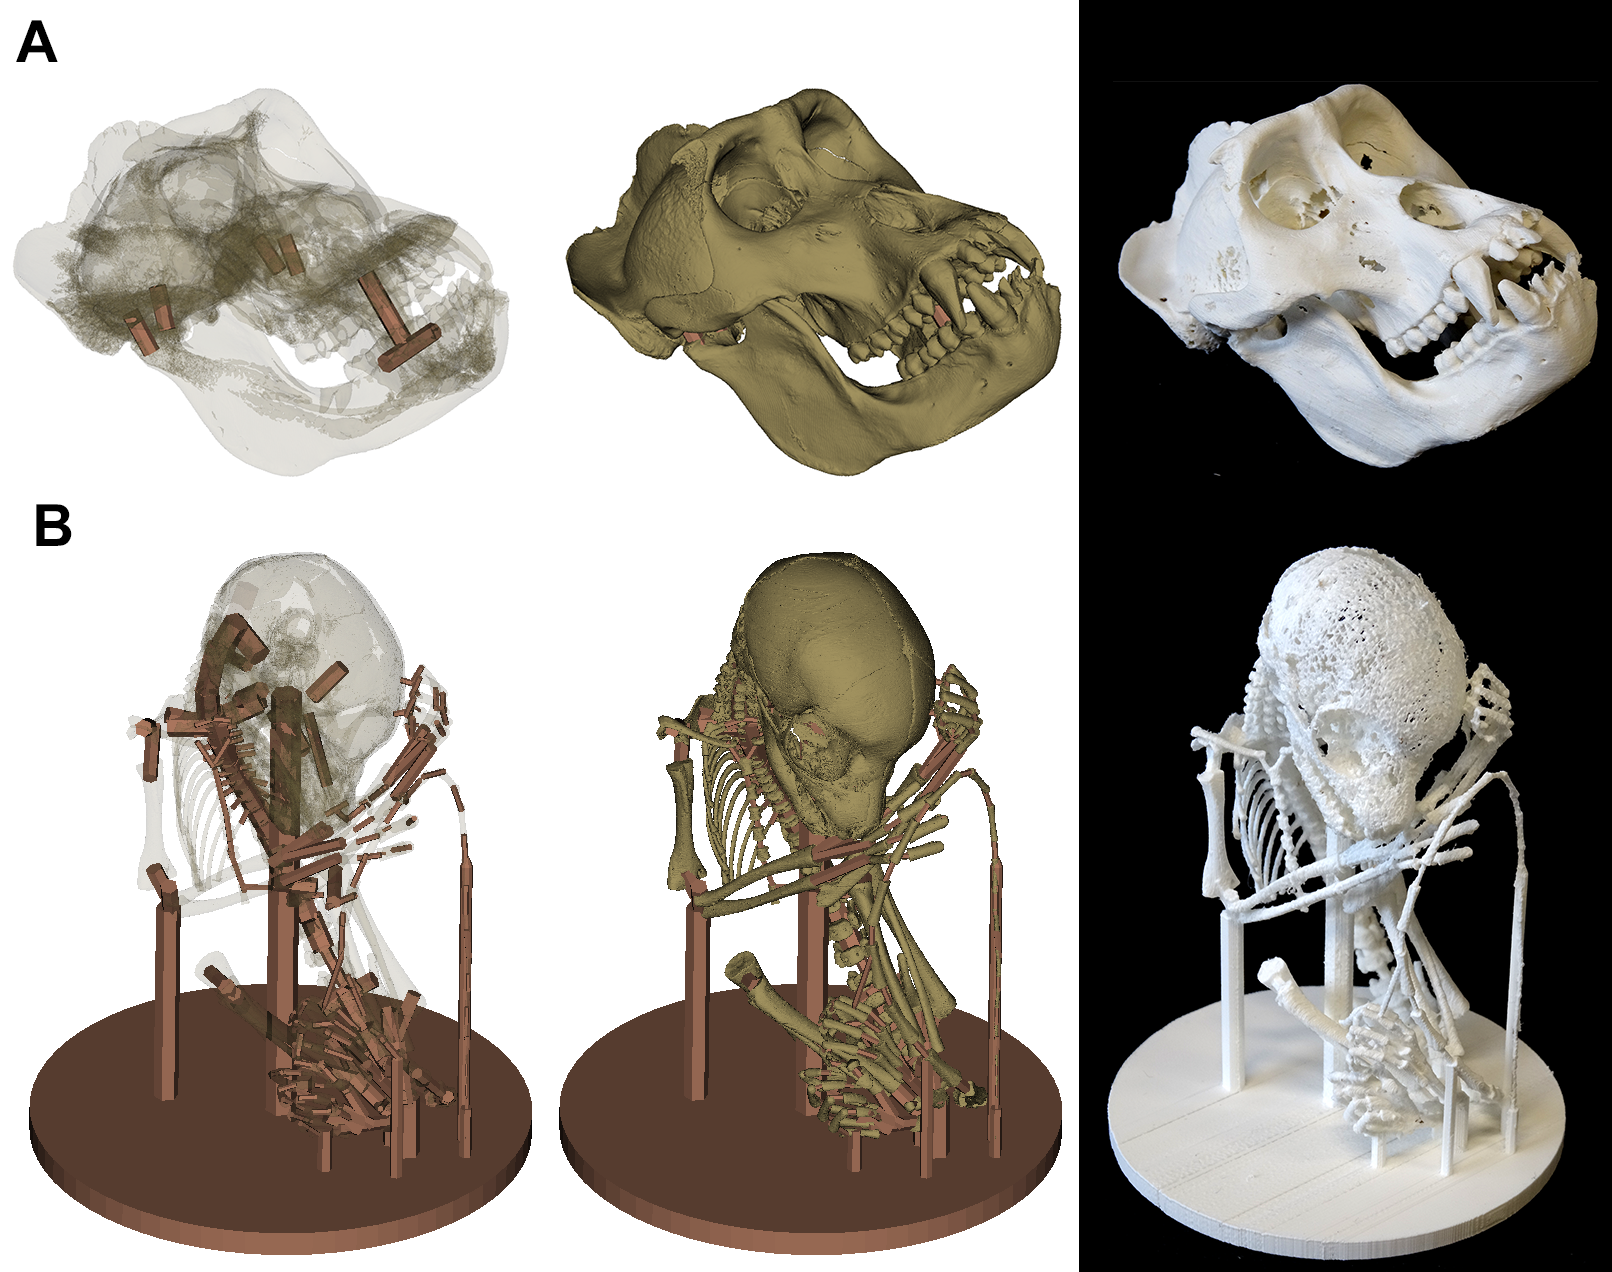
\includegraphics[scale=1.40]{images/09/create_3D_printing_support_surfaces/support_example.png} 
	\caption{Examples of 3D connective material usage. \textbf{A:} Cranium and mandible of \textit{Gorilla gorilla} (adult, male). Left: the 3D model of the skull is transparent, showing where the 3D connective cylinders have been placed in order to connect the mandible and the cranium. Middle: the same 3D model is rendered opaque. Right: 3D printed object. \textbf{B:} 3D model of the skeleton of a newborn \textit{Lemur catta}. The skeleton of this neonate specimen contains many non connected elements: many bones are not fully mineralized (skull bones, vertebrae) and most bones are separated in space. Left: the 3D model of the skeleton is transparent, showing the position of the many cylinders (two hundreds) of different lengths and diameters connecting the different bones. Right: 3D printed object. }
 \label{support_example}
\end{figure}

\subsection{Create cubic connective struts}
Different options are available, and in particular, the cubes / box-shaped struts can be given any desired width, height and depth (see Fig.  \ref{cubes_dialog} p.\pageref{cubes_dialog} and Fig. \ref{cubic} p.\pageref{cubic}). 

\begin{figure}
  \centering
  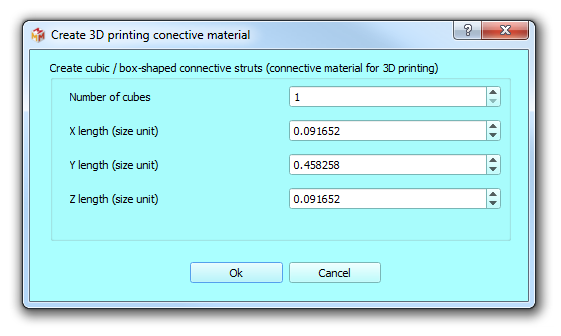
\includegraphics[scale=0.5]{images/09/create_3D_printing_support_surfaces/cubes_dialog.png} 
	\caption{Create cube dialog. The X,Y and Z lengths of the cubic / box-shaped connective struts can be defined here.}
 \label{cubes_dialog}
\end{figure}

\begin{figure}
  \centering
  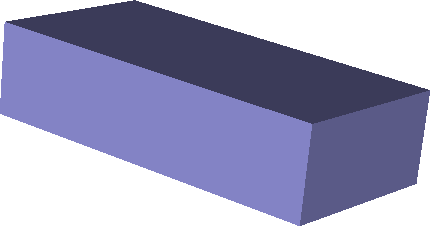
\includegraphics[scale=0.5]{images/09/create_3D_printing_support_surfaces/cubic.png} 
	\caption{Example of cubic connective strut.}
 \label{cubic}
\end{figure}
%\section{Delete small objects.}


